\documentclass[9pt,aspectratio=169]{beamer}
\usepackage{tikz}
\usetheme{default}
\setbeamertemplate{navigation symbols}{}
\title{Geometric uncertainty: experiments and bounds}
\subtitle{Generated interaction study}
\author{Research group}
\date{}
\year=2026\month=11\day=5
\newcommand{\fuzzlayerA}[1]{\textrm{#1}}
\newcommand{\fuzzlayerB}[1]{\fuzzlayerA{#1}}
\newcommand{\fuzzlayerC}[1]{\fuzzlayerB{#1}}
\newcommand{\fuzzterm}[1]{\fuzzlayerC{#1}}
\newcommand{\fuzzpair}[2]{\fuzzterm{#1}: #2}
\newcommand{\fuzzunit}{steps}
\let\fuzzoriginalunit\fuzzunit
\newcommand{\fuzzcoefficient}{4}
\newcommand{\fuzzscale}[2][\fuzzcoefficient]{#1\,#2}
\definecolor{fuzzpaint}{RGB}{255,0,255}
\definecolor{fuzzsecond}{RGB}{18,137,67}
\tikzset{fuzzvertex/.style={draw,rounded corners=1pt,fill=blue!10,inner sep=1pt,minimum width=.35cm,minimum height=.25cm}}
\begin{document}
\section{Geometric uncertainty}
\begin{frame}[t,shrink=5]{Geometric uncertainty}{Composed dependencies}
\fuzzpair{Experiment}{Timing: 12\fuzzunit; estimate $\fuzzscale{x}+\fuzzscale[2]{y}$.}\par
{\renewcommand{\fuzzunit}{cycles}\let\fuzzterm\textbf\fuzzpair{LocalScope}{Timing: 7\fuzzunit.}\par}
\fuzzpair{RestoredScope}{Timing: 11\fuzzunit.}\par
{\scriptsize\color{blue}\centering
\begin{description}
\item<1->[Stage 1] {\small\color{black}\raggedright
\textit{The next pass} must preserve the boundary conditions while revisiting dependent values.  The estimate is $x_i+x_{i+1}$.\par}
\item<2->[Stage 2] \begin{enumerate}
\item \[\begin{aligned}a+b&=c\\ d-e&=f\end{aligned}\]
\item 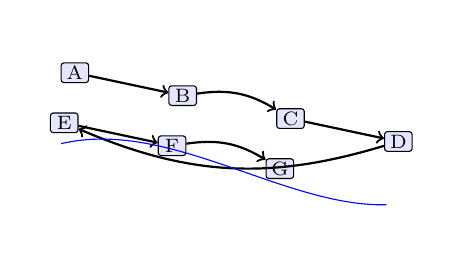
\begin{tikzpicture}[font=\scriptsize]
\begin{scope}[scale=1,rotate=-12]
\clip (-.4,-1) rectangle (4.700,.5);

\node[fuzzvertex] (g7n0) at (0.000,0) {A};
\node[fuzzvertex] (g7n1) at (1.400,0) {B};
\node[fuzzvertex] (g7n2) at (2.800,0) {C};
\node[fuzzvertex] (g7n3) at (4.200,0) {D};
\node[fuzzvertex] (g7n4) at (0.000,-0.65) {E};
\node[fuzzvertex] (g7n5) at (1.400,-0.65) {F};
\node[fuzzvertex] (g7n6) at (2.800,-0.65) {G};
\begin{scope}[xshift=.5pt,yshift=-.5pt]
\draw<2->[->,thick] (g7n0) -- (g7n1);
\draw<2->[->,thick] (g7n1) to[bend left=20] (g7n2);
\draw<2->[->,thick] (g7n2) -- (g7n3);
\draw<2->[->,thick] (g7n3) to[bend left=20] (g7n4);
\draw<2->[->,thick] (g7n4) -- (g7n5);
\draw<2->[->,thick] (g7n5) to[bend left=20] (g7n6);
\draw[blue] (0,-.9) .. controls (1.260,-.3) and (2.940,-1.1) .. (4.200,-.8);
\end{scope}
\end{scope}
\end{tikzpicture}
\end{enumerate}
\par
\textbf{We compare the} proposed solution with a reference computed from the complete input. We compare the proposed solution with a reference computed from the complete input. The estimate is $\sum_{i=1}^{n}x_i$.
\par
\alt<2-3>{\begin{tabular}{lrr}Method&Cost&Error\\\hline
Cached0&16&21\\
Cached1&2&26\\
Cached2&17&5\\
Cached3&10&17\\
\end{tabular}}{Alternative estimate $x_0$.}
\end{description}\par}
\par 
\begin{tikzpicture}[font=\scriptsize]
\fill<2-3>[fuzzpaint] (0,0) rectangle (.8,.3);
\fill<3->[fuzzsecond] (1,0) rectangle (1.8,.3);
\node[anchor=west] at (2,0.15) {Witness};
\end{tikzpicture}
\only<4>{}
\end{frame}
\renewcommand{\fuzzunit}{us}
\renewcommand{\fuzzcoefficient}{2}
\renewcommand{\fuzzterm}[1]{{\textrm{#1}}}
\section{Message passing}
\begin{frame}[t]{Cache invalidation}
\fuzzpair{MacroStageB}{Timing: 12\fuzzunit, retained: 9\fuzzoriginalunit.}\par
{\renewcommand{\fuzzunit}{local}\fuzzpair{FrameLocal}{Timing: 5\fuzzunit.}\par}
\fuzzpair{FrameRestored}{Timing: 8\fuzzunit; estimate $\fuzzscale{x}$.}\par
\begin{columns}[T]\begin{column}{.46\textwidth}A narrow column can change line breaking even when the underlying expression is unchanged.\end{column}\begin{column}{.46\textwidth}\begin{itemize}\item Input state\item Updated state\end{itemize}\end{column}\end{columns}
\end{frame}
\end{document}
